% ============================================================
%  CHAPITRE 2 : La turbulence en mécanique des fluides numérique
% ============================================================
\chapter{La turbulence en mécanique des fluides numérique}
\label{chap:turbulence}

\section{Introduction}
\label{sec:introduction_turbulence}

La turbulence désigne l'état de l'écoulement d'un fluide, liquide ou gaz, dont la vitesse possède un caractère tourbillonnaire et une orientation variable constamment dans l'espace, ce qui ne permet pas de prévoir son comportement de manière déterministe \cite{tennekes1972first}. Les écoulements turbulents se caractérisent par :
\begin{itemize}
    \item Le désordre et l'irrégularité de l'écoulement. \item Un caractère tridimensionnel et non-linéaire. \item La présence de tourbillons de différentes échelles avec un transfert d'énergie des plus grands vers les plus petits \cite{pope2000turbulent}, comme illustré à la Figure~\ref{fig:turbulent}. \end{itemize}

\begin{figure}[H]
    \centering
    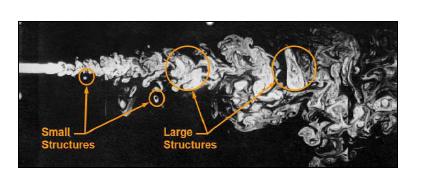
\includegraphics[width=0.45\textwidth]{figures/figure2_2.png}
    \caption{Écoulement turbulent.}
    \label{fig:turbulent}
\end{figure}

L'origine du désordre caractérisant l'écoulement repose sur le terme non-linéaire de l'équation de Navier-Stokes qui est le terme inertiel de transport par convection. Ainsi, plus le nombre de Reynolds est grand, plus ce terme aura du poids dans la dynamique et plus l'écoulement sera complexe et turbulent \cite{davidson2015turbulence}. Le nombre de Reynolds est donné comme suit : \cite{reynolds1883experimental}

\begin{equation}
Re = \frac{V \times L}{\nu}
\label{eq:reynolds}
\end{equation}

\begin{itemize}
    \item[--] \(V\) : la vitesse caractéristique de l'écoulement \([m/s]\)
    \item[--] \(L\) : la longueur caractéristique du domaine \([m]\)
    \item[--] \(\nu\) : la viscosité cinématique du fluide \([m^2/s]\)
\end{itemize}

Le tableau ci-dessous illustre, à titre d'exemple, quelques valeurs critiques de $Re$ pour différentes géométries :

\begin{table}[H]
    \centering
    \caption{Exemples de valeurs critiques du nombre de Reynolds}
    \label{tab:reynolds_critique}
    \begin{tabular}{|l|c|c|}
        \hline
        \textbf{Géométrie} & \textbf{Longueur caractéristique L} & \textbf{Re critique} \\
        \hline
        Écoulement en conduite & Diamètre (D) & $\approx 2300$ \\
        \hline
        Plaque plane (couche limite) & Longueur de la plaque (x) & $\approx 5\times10^5$ \\
        \hline
        Écoulement autour d'une sphère & Diamètre (D) & $\approx 3\times10^5$ \\
        \hline
        Entre deux plaques parallèles & Distance entre plaques (h) & $\approx 1000$ \\
        \hline
    \end{tabular}
\end{table}

\section{Les approches de modélisation de la turbulence}
\label{sec:approches_turbulence}

La modélisation de la turbulence est une branche de la mécanique des fluides utilisée pour prédire le comportement d'un écoulement dans lequel tout ou partie du fluide est turbulent. Malgré des efforts importants de recherche depuis plus d'un siècle, la modélisation des écoulements turbulents demeure un défi à relever \cite{wilcox2006turbulence}. Il existe principalement trois axes de recherche : \cite{sagaut2006large}

\subsection{Simulation numérique directe (DNS)}
\label{subsec:dns}

La DNS permet de résoudre directement les équations de Navier-Stokes (voir équation~\eqref{eq:navier_stokes}) sans aucune modélisation. Elle présente ainsi l'avantage de donner accès à toutes les quantités instantanées considérées dans l'écoulement. Tous les mouvements doivent être résolus depuis les plus petites échelles dissipatives jusqu'à l'échelle intégrale, comme illustré à la Figure~\ref{fig:dns_jet}. Le nombre de mailles est alors très important, ce qui engendre des temps de calcul extrêmement longs \cite{moin1998direct}. La capacité et la performance des calculateurs actuels ne cessent de progresser mais ne permettent pas encore de sonder des écoulements complexes dans un contexte industriel.

\begin{figure}[H]
    \centering
    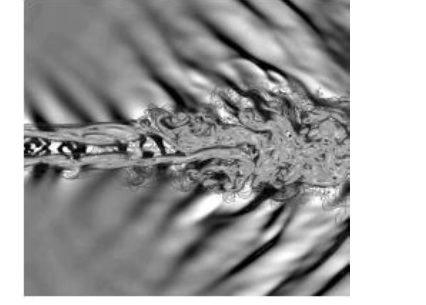
\includegraphics[width=0.6\textwidth]{figures/figure2_3.png}
    \caption{DNS d'un jet d'air issu d'une tuyère \cite{moin1998direct}.}
    \label{fig:dns_jet}
\end{figure}

\subsection{Simulation des grandes échelles (LES~: Large Eddy Simulation)}
\label{subsec:les}

La LES est une méthode numérique intermédiaire entre la DNS et les méthodes statistiques \cite{lesieur2005large}. Elle consiste à appliquer un filtre spatial aux équations de Navier-Stokes (voir équation~\eqref{eq:navier_stokes}) en tout point du domaine. Le champ filtré est défini par :

\begin{equation}
\bar{\Phi}(x) = \int_D \Phi(x') G(x, x') dx'
\label{eq:filtre_les}
\end{equation}

\begin{itemize}
    \item[--] \(\bar{\Phi}(x)\) : le champ filtré (représentant les grandes échelles)
    \item[--] \(\Phi(x')\) : le champ instantané non filtré
    \item[--] \(G(x, x')\) : le noyau (fonction) du filtre spatial
    \item[--] \(D\) : le domaine de filtrage
\end{itemize}

Le filtre sépare les grandes échelles (simulées) des petites structures (modélisées), comme illustré à la Figure~\ref{fig:les_anneaux}. On suppose ici que le comportement de ces dernières ne dépend pas de la géométrie et est universel. La LES est moins coûteuse que la DNS, mais reste très exigeante en ressources de calcul, ce qui limite encore son application industrielle courante \cite{piomelli1999large}.

\begin{figure}[H]
    \centering
    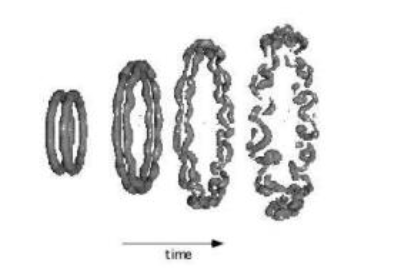
\includegraphics[width=0.6\textwidth]{figures/figure2_4.png}
    \caption{LES de la collision axiale de deux anneaux tourbillonnaires \cite{piomelli1999large}.}
    \label{fig:les_anneaux}
\end{figure}

\subsection{Modélisation statistique (RANS)}
\label{subsec:rans}

La méthode RANS (Reynolds-Averaged Navier-Stokes) est une approche qui consiste à mettre de côté le mouvement instantané du fluide, afin d'exprimer les équations du champ moyen en se servant de la décomposition de Reynolds. Chaque variable est décomposée en une partie moyenne et une partie fluctuante \cite{reynolds1895dynamical} :

\begin{equation}
\phi(x_i, t) = \overline{\phi}(x_i) + \phi'(x_i, t)
\label{eq:decomposition_reynolds}
\end{equation}

\begin{figure}[H]
    \centering
    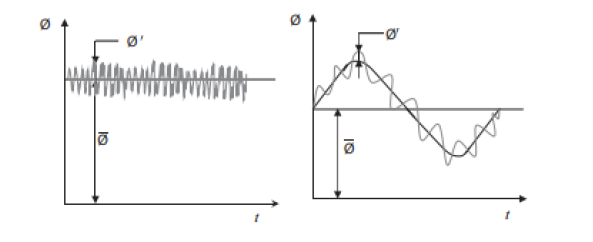
\includegraphics[width=0.6\textwidth]{figures/figure2_5.png}
    \caption{Décomposition des variables selon l'approche RANS \cite{reynolds1895dynamical}.}
    \label{fig:decomposition_reynolds}
\end{figure}

En introduisant cette décomposition dans les équations de Navier-Stokes et en prenant la moyenne, on obtient les équations RANS (Reynolds-Averaged Navier-Stokes), dont le principe est illustré à la Figure~\ref{fig:decomposition_reynolds}. Ce processus fait apparaître de nouvelles inconnues : les \textbf{tensions de Reynolds} (\( -\rho \overline{u_i' u_j'} \)), qui représentent l'influence des fluctuations turbulentes sur l'écoulement moyen \cite{hinze1975turbulence}.

\subsection{Remarques sur les trois approches}
\label{subsec:remarques_approches}

Pour une modélisation précise, il faut prévoir des maillages très fins, ce qui nécessite des coûts et des temps très importants. C'est pour cela qu'on préfère l'approche statistique car elle est plus rapide et moins coûteuse \cite{rodi1993turbulence}. Le tableau suivant compare les différentes approches de modélisation : \cite{durbin2010statistical}

\begin{table}[H]
    \centering
    \caption{Comparaison des approches de modélisation de la turbulence}
    \label{tab:comparaison_approches}
    \small
    \begin{tabular}{|l|p{3.5cm}|p{2.5cm}|p{1.8cm}|p{3.5cm}|}
        \hline
        \textbf{Approche} & \textbf{Résolution des tourbillons} & \textbf{Coût de calcul} & \textbf{Précision} & \textbf{Applications} \\
        \hline
        RANS & Tous modélisés & Faible & Moyenne & Industrielles courantes \\
        \hline
        LES & Grands résolus, petits modélisés & Élevé & Bonne & Recherche, écoulements complexes \\
        \hline
        DNS & Tous résolus & Extrêmement élevé & Excellente & Recherche fondamentale \\
        \hline
    \end{tabular}
\end{table}

\section{Classification des modèles de turbulence}
\label{sec:classification_modeles}

Le système formé par les équations RANS n'est pas fermé, car on dispose de quatre équations mais dix inconnues, ce sont les tensions de Reynolds qui posent le problème. L'enjeu est de trouver une relation liant les tensions de Reynolds au champ de vitesse moyen \cite{launder1972lectures}.

\subsection{Modèle à viscosité turbulente}
\label{subsec:viscosite_turbulente}

Boussinesq fut le premier à introduire la notion de viscosité turbulente en proposant une relation en analogie avec celle de Newton pour les contraintes de viscosité moléculaire \cite{boussinesq1877essai}. Schématiquement cela revient à poser une relation linéaire entre les contraintes turbulentes (contraintes de Reynolds) et le gradient de vitesse moyen : \cite{schmitt2007boussinesq}

\begin{equation}
-\rho \overline{u_i' u_j'} = \mu_t \left( \frac{\partial \overline{u_i}}{\partial x_j} + \frac{\partial \overline{u_j}}{\partial x_i} \right) - \frac{2}{3} \rho k \delta_{ij}
\label{eq:boussinesq}
\end{equation}

où les termes sont définis comme suit :
\begin{itemize}
    \item[--] \(\mu_t\) : la viscosité dynamique turbulente \([Pa \cdot s]\)
    \item[--] \(k\) : l'énergie cinétique turbulente \([m^2/s^2]\)
    \item[--] \(\delta_{ij}\) : le tenseur de Kronecker (\(\delta_{ij} = 1\) si \(i=j\), 0 sinon)
    \item[--] \(\overline{u_i}\), \(\overline{u_j}\) : les composantes de la vitesse moyenne
\end{itemize}

\subsection{Le modèle de longueur de mélange -- modèle de Prandtl}
\label{subsec:longueur_melange}

Une étude dimensionnelle montre que la viscosité turbulente est proportionnelle à une échelle de longueur $l$ et une échelle de vitesse $u$ représentatives de l'agitation turbulente \cite{prandtl1925bericht}. Prandtl a proposé le modèle de longueur de mélange dans lequel la viscosité cinématique turbulente \( \nu_t \) est directement reliée au gradient de vitesse moyenne par l'intermédiaire d'une longueur \( l_m \) appelée longueur de mélange : \cite{prandtl1945uber}

\begin{equation}
\nu_t = l_m^2 \left| \frac{\partial \bar{u}}{\partial y} \right|
\label{eq:longueur_melange}
\end{equation}

Avec \( l_m = \kappa y \) et \( \kappa = 0{,}41 \) la constante de Von Karman.

\section{Modèles de fermeture des approches statistiques à deux équations de transport}
\label{sec:modeles_deux_equations}

Plusieurs modèles à deux équations ont été développés pour représenter les deux échelles indépendamment. Ils sont largement utilisés dans l'industrie \cite{hanjalic2011modelling}.

\subsection{Modèle de fermeture \texorpdfstring{$k$-$\varepsilon$}{k-epsilon}}
\label{subsec:modele_k_epsilon}

Ce modèle a été établi par Jones et Launder \cite{jones1972prediction}. Il relie les grandeurs caractéristiques de la turbulence : énergie cinétique turbulente $k$, taux de dissipation $\varepsilon$ et viscosité turbulente \( \mu_t \). Les équations de transport de $k$ et $\varepsilon$ sont \cite{launder1974application} :

\begin{align}
\frac{\partial}{\partial t} (\rho k) + \frac{\partial}{\partial x_j} (\rho u_j k) &= \frac{\partial}{\partial x_j} \left[ \left( \mu + \frac{\mu_t}{\sigma_k} \right) \frac{\partial k}{\partial x_j} \right] + P_k - \rho \varepsilon \label{eq:transport_k} \\
\frac{\partial}{\partial t} (\rho \varepsilon) + \frac{\partial}{\partial x_j} (\rho u_j \varepsilon) &= \frac{\partial}{\partial x_j} \left[ \left( \mu + \frac{\mu_t}{\sigma_\varepsilon} \right) \frac{\partial \varepsilon}{\partial x_j} \right] + C_{\varepsilon 1} \frac{\varepsilon}{k} P_k - C_{\varepsilon 2} \frac{\rho \varepsilon^2}{k} \label{eq:transport_epsilon}
\end{align}

La viscosité turbulente est donnée par \( \mu_t = \rho C_\mu \frac{k^2}{\varepsilon} \). Les constantes du modèle standard sont : \( C_\mu = 0,09 \), \( C_{\varepsilon 1} = 1,44 \), \( C_{\varepsilon 2} = 1,92 \), \( \sigma_k = 1,0 \), \( \sigma_\varepsilon = 1,3 \) \cite{launder1974numerical}.

\subsection{Modèle de fermeture \( k-\omega \)}
\label{subsec:modele_k_omega}

Le modèle \( k-\omega \) de Wilcox \cite{wilcox1988reassessment} utilise le paramètre \( \omega \), le taux de dissipation spécifique défini par \( \omega = \varepsilon/k \). La viscosité turbulente devient \( \mu_t = \rho \frac{k}{\omega} \). Les équations de transport sont \cite{wilcox2008formulation} :

\begin{align}
\frac{\partial}{\partial t} (\rho k) + \frac{\partial}{\partial x_j} (\rho u_j k) &= \frac{\partial}{\partial x_j} \left[ \left( \mu + \frac{\mu_t}{\sigma_k} \right) \frac{\partial k}{\partial x_j} \right] + P_k - \beta^* \rho k \omega \label{eq:transport_k_omega} \\
\frac{\partial}{\partial t} (\rho \omega) + \frac{\partial}{\partial x_j} (\rho u_j \omega) &= \frac{\partial}{\partial x_j} \left[ \left( \mu + \frac{\mu_t}{\sigma_\omega} \right) \frac{\partial \omega}{\partial x_j} \right] + \alpha \frac{\omega}{k} P_k - \beta \rho \omega^2 \label{eq:transport_omega}
\end{align}

\subsection{Modèle de fermeture \( k-\omega \) SST}
\label{subsec:modele_k_omega_sst}

Menter \cite{menter1994two} a proposé un modèle hybride combinant les avantages des modèles \( k-\omega \) près des parois et \( k-\varepsilon \) loin des parois. Le modèle \( k-\omega \) SST (Shear Stress Transport) utilise une fonction de commutation \( F_1 \) pour basculer entre les deux formulations \cite{menter2003ten} :

\begin{equation}
\mu_t = \frac{a_1 \rho k}{\max(a_1 \omega, S F_2)}
\label{eq:mu_t_sst}
\end{equation}

\begin{itemize}
    \item[--] \(a_1 = 0{,}31\) : constante du modèle SST
    \item[--] \(\rho\) : masse volumique du fluide \([kg/m^3]\)
    \item[--] \(k\) : énergie cinétique turbulente \([m^2/s^2]\)
    \item[--] \(\omega\) : taux de dissipation spécifique \([1/s]\)
    \item[--] \(S\) : invariant du tenseur des taux de déformation \([1/s]\)
    \item[--] \(F_2\) : seconde fonction de commutation du modèle SST
\end{itemize}

Ce modèle sera privilégié pour notre étude car il offre une bonne précision dans les zones à forts gradients de vitesse, ce qui est essentiel pour modéliser correctement les écoulements dans les évacuateurs de crues et les vidanges de fond.


% SECTION 2.5 : CONCLUSION
\section{Conclusion}
\label{sec:conclusion_chap2}

En définitive, bien que la turbulence soit un phénomène omniprésent dans la nature et le quotidien, elle reste difficile à définir avec précision en raison de son caractère chaotique et imprévisible. Ce comportement tourbillonnaire, en perpétuelle variation de forme, de position et d'intensité, traduit la complexité du régime turbulent. Pour notre étude, le modèle \( k-\omega \) SST sera privilégié car il combine robustesse et précision.